\documentclass{beamer}
\usepackage{tikz}
\usepackage{hyperref}
\beamertemplatenavigationsymbolsempty

\usetikzlibrary{shapes}
\usetikzlibrary{shapes.misc}
\usetikzlibrary{positioning}
\usetikzlibrary{decorations.pathmorphing}
\usetikzlibrary{decorations.pathreplacing}
\usetikzlibrary{decorations.shapes}
\usetikzlibrary{calc}
\usetikzlibrary{arrows}
\usetikzlibrary{automata}
\usetikzlibrary{external}

\tikzexternalize[prefix=doc/presentation-figures/]

\title[Omics data integration]{Integrative causality analysis of genetic,
epigenetic, and transcriptomic data in a large cohort}
\author[R. McCloskey \& S. Mostafavi]
    {Rosemary McCloskey and Sara Mostafavi \\\hfill\\
     \small
     \url{rmcclosk.math@gmail.com} \\
     \url{http://slideshare.net/rmcclosk/omics-integration}
     \normalsize}
\date{March 27, 2015}

\usetheme{Madrid}
\usecolortheme{crane}

\begin{document}

\maketitle

\begin{frame}
    \frametitle{Motivation}
    \begin{itemize}
        \item genetic, epigenetic, and transcriptomic data provide snapshots of
            cellular processes
        \uncover<2->{
        \item usually one data type is studied at a time, in relation to a
            phenotype or disease
        }
    \begin{center}
        \vspace{-0.5cm}
        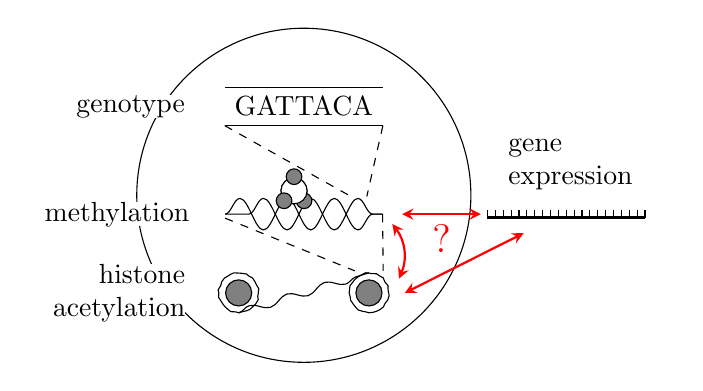
\begin{tikzpicture}
    \node (g) {GATTACA};
    \draw (g.north west) -- (g.north east);
    \draw (g.south west) -- (g.south east);

    \node [below left= of g.south] (m1) {};
    \node [below right= of g.south] (m2) {};
    \draw [decorate, decoration={snake, segment length=6mm, amplitude=2mm}] (m1) -- (m2);
    \draw [decorate, decoration={snake, segment length=6mm, amplitude=2mm, pre length=3mm}] (m1) -- (m2);
    \node [right=1cm of m1.north, anchor=south, circle, draw, fill=white] (me) { };
    \node [below right=-0.1 of me.south east, anchor=north west, circle, draw, fill=gray, inner sep=2pt] { };
    \node [right=1cm of m1.north, anchor=south, circle, draw, fill=white] (me) { };
    \node [below left=-0.1 of me.south west, anchor=north east, circle, draw, fill=gray, inner sep=2pt] { };
    \node [above=-0.1 of me.north, anchor=south, circle, draw, fill=gray, inner sep=2pt] { };

    \node [below= of m1.east, anchor=west, circle, draw, fill=gray] (a1) { };
    \node [below= of m2.west, anchor=east, circle, draw, fill=gray] (a2) { };
    \node [above=0 of a1.center, anchor=center, circle, draw, decorate,
           decoration={random steps, amplitude=0.1mm, segment length=0.5mm}, 
           inner sep=5pt] (a1out) { };
    \node [above=0 of a2.center, anchor=center, circle, draw, decorate,
           decoration={random steps, amplitude=0.1mm, segment length=0.5mm}, 
           inner sep=5pt] (a2out) { };
    \draw [decorate, decoration={snake, amplitude=0.5mm, segment length=5mm}]
          (a1out.south) -- (a2out.north);

    \draw [dashed] (g.south west) -- ($(m2.north west) + (-4mm, 1mm)$);
    \draw [dashed] (g.south east) -- ($(m2.north west) + (-2mm, 1mm)$);

    \draw [dashed] (m1) -- ($(a2out.north west) + (0mm, 1mm)$);
    \draw [dashed] (m2.west) -- ($(a2out.north east) + (0mm, 1mm)$);

    \node [circle, draw, above=of g.center, anchor=north, inner sep=1.5cm] { };

    \node [right=1cm of m2, inner sep=1pt] (e1) { };
    \node [right=2cm of e1, inner sep=1pt] (e2) { };
    \draw [decorate, decoration={ticks, amplitude=0.5mm, segment length=1mm}] (e1) -- (e2);
    \draw [thick] (e1.south east) -- (e2.south west);

    \uncover<3-> {
    \draw [<->, >=stealth, thick, color=red] (e1) -- node [auto, color=red] {\Large{?}} (m2);
    \draw [<->, >=stealth, thick, color=red] ($(e1.south) + (5mm, -2mm)$) -- 
    ($(a2out.east) + (2mm, 0mm)$);
    \path [bend left, draw, <->, >=stealth, thick, color=red] (m2.south) to 
    ($(a2out.north east) + (2mm, 0)$);
    }

    \node [above right=2mm of e1, text width=2cm] {gene \\ expression};
    \node [left=2mm of m1, fill=white, inner sep=0pt, align=right] {methylation};
    \node [left=5mm of a1, fill=white, inner sep=0pt, text width=2cm,
    align=right] {histone \\ acetylation};
    \node [left=5mm of g.west, fill=white, inner sep=0pt, align=right] {genotype};
\end{tikzpicture}

    \end{center}
        \uncover<3->{
        \item \textbf{how do these data fit together?}
        }
    \end{itemize}
\end{frame}

\begin{frame}{The data}
    \begin{columns}
        \begin{column}{0.35\textwidth}
            \begin{itemize}
                \item large cohort designed to study cognitive decline and
                    Alzheimer's disease
                \uncover<2->{
                \item genotype, gene expression, DNA methylation, and histone
                    acetylation (CHiP-seq) data 
                }
                \uncover<3->{
                \item 392 individuals with all four data types were used for
                    this analysis
                }
            \end{itemize}
        \end{column}
        \begin{column}{0.7\textwidth}
            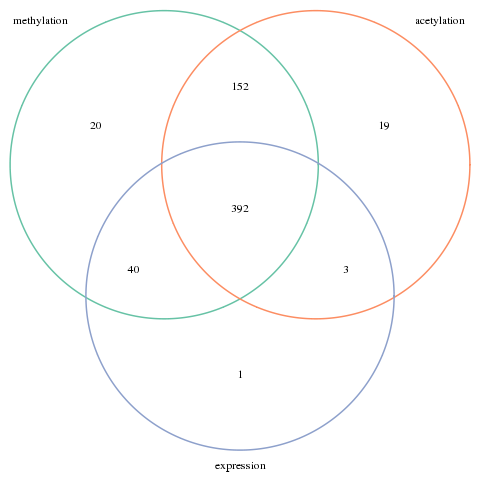
\includegraphics[width=\linewidth]{doc/figures/datatypes_venn}
        \end{column}
    \end{columns}
\end{frame}

\begin{frame}{Quantitative trait loci (QTLs)}
    \begin{columns}
        \begin{column}{0.4\textwidth}
            \begin{itemize}
                \item a QTL is a genetic locus correlated with a phenotype
                \uncover<2->{
                \item we are interested in QTLs for gene expression (eQTLs),
                    histone acetylation (aceQTLs), and methylation (meQTLs)
                }
                \uncover<3->{
                \item QTLs provide a tool to study interaction between other
                    molecular phenotypes
                }
            \end{itemize}
        \end{column}
        \begin{column}{0.65\textwidth}
            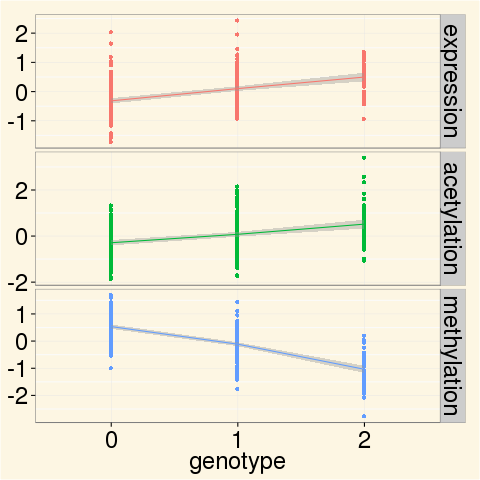
\includegraphics[width=\linewidth]{doc/figures/qtl_example}
        \end{column}
    \end{columns}
\end{frame}

\begin{frame}{Identifying QTLs}
    \begin{center}
        \tikzexternaldisable
        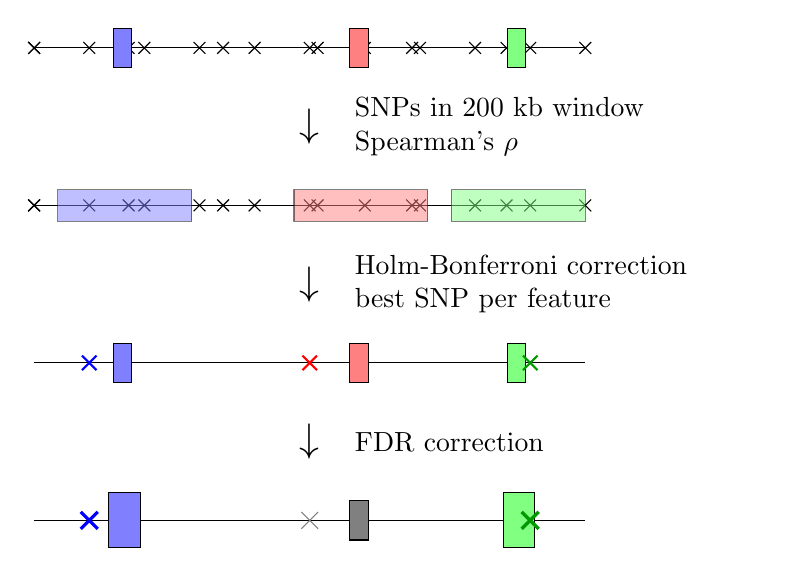
\begin{tikzpicture}
    [feature/.style={rectangle, draw, minimum height=5mm},
     cross/.style={cross out, draw, minimum size=2*(#1-\pgflinewidth), 
     inner sep=0pt, outer sep=0pt},
     cross/.default={1.2mm}]
    \coordinate (5prime);
    \coordinate [right=7cm of 5prime] (3prime);
    \draw (5prime) -- (3prime);
    \draw [decorate, decoration={crosses, segment length=7mm, shape size=1.5mm}]
          (5prime) -- (3prime);
    \draw [decorate, 
           decoration={crosses, segment length=12mm, shape size=1.5mm}] 
          (5prime) -- (3prime);
    \node [feature, right=1cm of 5prime, fill=blue!50!white] (f1) { };
    \node [feature, right=4cm of 5prime, fill=red!50!white] (f2) { };
    \node [feature, right=6cm of 5prime, fill=green!50!white] (f3) { };

    \uncover<2->{

    \coordinate [below=2cm of 5prime] (5prime2);
    \coordinate [below=2cm of 3prime] (3prime2);
    \draw (5prime2) -- (3prime2);
    \draw [decorate, decoration={crosses, segment length=7mm, shape size=1.5mm}]
          (5prime2) -- (3prime2);
    \draw [decorate, 
           decoration={crosses, segment length=12mm, shape size=1.5mm}] 
          (5prime2) -- (3prime2);
    \draw [fill=blue!50!white, opacity=0.5] ($(5prime2) + (0.3cm, 0.2cm)$) 
          rectangle ($(5prime2) + (2cm, -0.2cm)$);
    \draw [fill=red!50!white, opacity=0.5] ($(5prime2) + (3.3cm, 0.2cm)$) 
          rectangle ($(5prime2) + (5cm, -0.2cm)$);
    \draw [fill=green!50!white, opacity=0.5] ($(5prime2) + (5.3cm, 0.2cm)$) 
          rectangle ($(5prime2) + (7cm, -0.2cm)$);
    \path (5prime) -- node (mid1) {\Large{$\downarrow$}} (3prime2);
    \node [right=2mm of mid1, text width=5cm] {SNPs in 200 kb window \\
    Spearman's $\rho$};

    }\uncover<3->{

    \coordinate [below=2cm of 5prime2] (5prime3);
    \coordinate [below=2cm of 3prime2] (3prime3);
    \draw (5prime3) -- (3prime3);
    \node [feature, right=1cm of 5prime3, fill=blue!50!white] (f1) { };
    \node [feature, right=4cm of 5prime3, fill=red!50!white] (f2) { };
    \node [feature, right=6cm of 5prime3, fill=green!50!white] (f3) { };
    \node [cross, blue, thick] at ($(5prime3) + (7mm, 0mm)$) { };
    \node [cross, red, thick] at ($(5prime3) + (35mm, 0mm)$) { };
    \node [cross, green!60!black, thick] at ($(5prime3) + (63mm, 0mm)$) { };
    \path (5prime2) -- node (mid2) {\Large{$\downarrow$}} (3prime3);
    \node [right=2mm of mid2, text width=5cm] {Holm-Bonferroni correction \\ best SNP per feature};

    }\uncover<4->{

    \coordinate [below=2cm of 5prime3] (5prime4);
    \coordinate [below=2cm of 3prime3] (3prime4);
    \draw (5prime4) -- (3prime4);
    \node [feature, minimum height=7mm, minimum width=4mm, right=1.15cm of
    5prime4, anchor=center, fill=blue!50!white] (f1) { };
    \node [feature, right=4cm of 5prime4, fill=gray] (f2) { };
    \node [feature, right=5.95cm of 5prime4, minimum height=7mm, minimum width=4mm, fill=green!50!white] (f3) { };
    \node [cross, cross=1.5mm, blue, very thick] at ($(5prime4) + (7mm, 0mm)$) { };
    \node [cross, gray] at ($(5prime4) + (35mm, 0mm)$) { };
    \node [cross, cross=1.5mm, green!60!black, very thick] at ($(5prime4) + (63mm, 0mm)$) { };
    \path (5prime3) -- node (mid3) {\Large{$\downarrow$}} (3prime4);
    \node [right=2mm of mid3] {FDR correction};

    }
\end{tikzpicture}

        \tikzexternalenable
    \end{center}
\end{frame}

\begin{frame}{Removing Principal Components}
    \begin{columns}
    \begin{column}{0.4\textwidth}
        \begin{itemize}
            \item technical, environmental, and biological covariates can swamp
                out QTL effects
            \uncover<2->{
            \item correct by removing principal components 
            }\uncover<3->{
            \item number of peaks with a QTL plateaus at 10 PCs, while genes and
                CpGs continue to increase
            }\uncover<4->{
            \item for this analysis, removed 10 PCs from all data
            }
        \end{itemize}
    \end{column}
    \begin{column}{0.6\textwidth}
        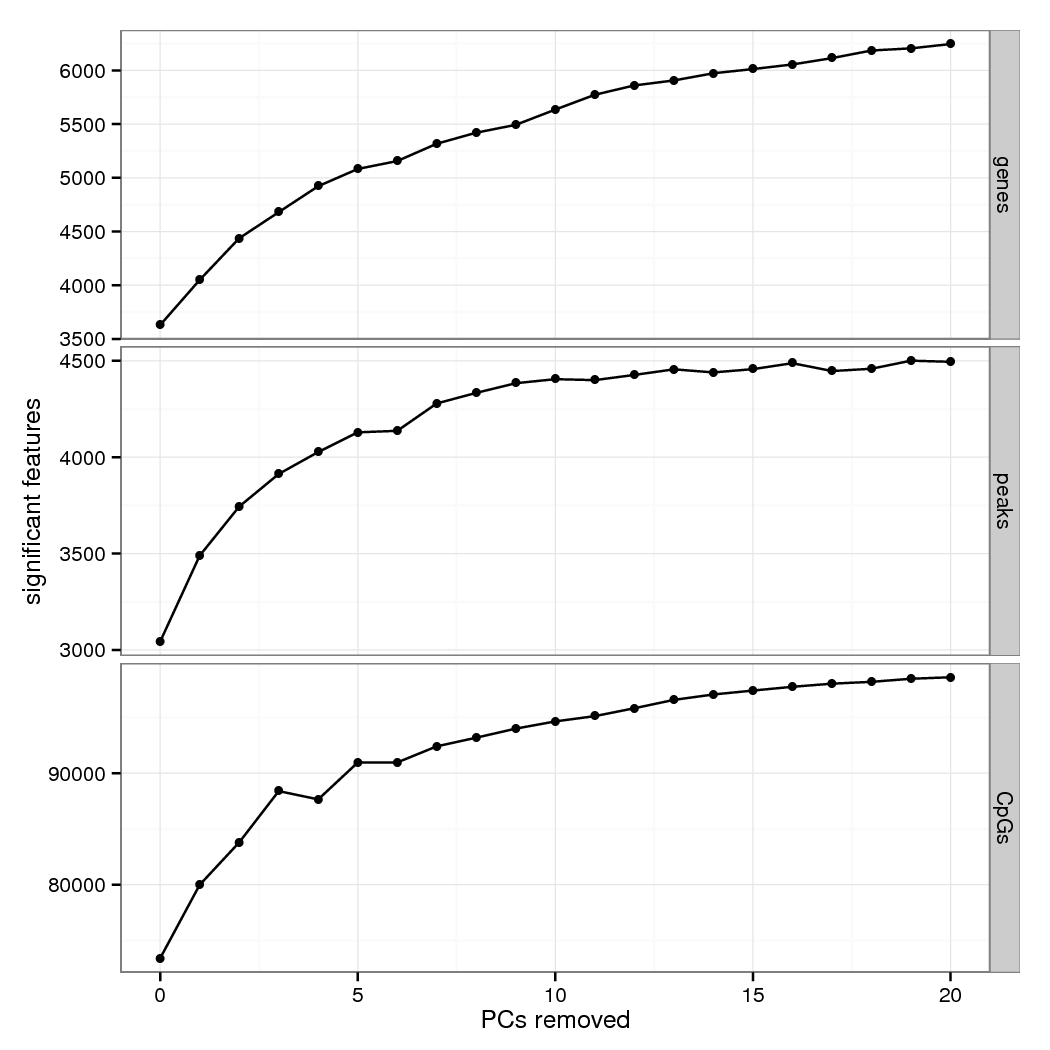
\includegraphics[width=\linewidth]{doc/figures/qtl_pca}
    \end{column}
    \end{columns}
\end{frame}

\begin{frame}{Identifying multi-QTLs}
\begin{columns}
    \begin{column}{0.5\textwidth}
        \begin{itemize}
            \item By intersecting QTL sets, found 240 gene, CpG, and peak
                triples which shared the same QTL 
        \end{itemize}
        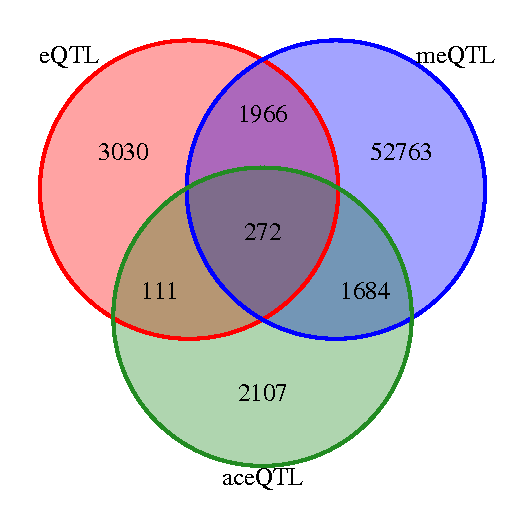
\includegraphics[width=\linewidth]{doc/figures/qtl_venn}
    \end{column}
    \pause
    \begin{column}{0.5\textwidth}
        \begin{itemize}
            \item Also assessed QTL overlap using $\pi_0$ approach 
        \end{itemize}
        \vspace{-0.3cm}
        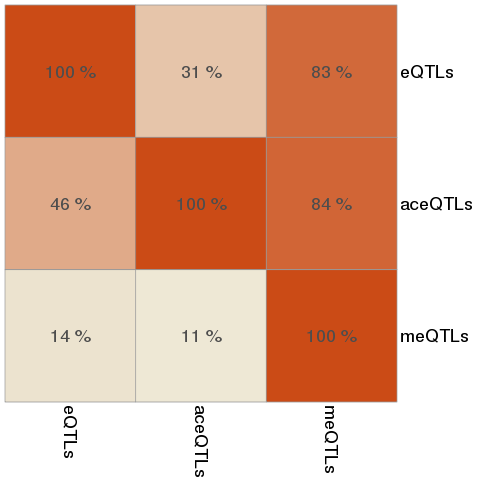
\includegraphics[width=\linewidth]{doc/figures/qtl_overlap}
        \vspace{-0.5cm}
    \end{column}
\end{columns}
\end{frame}

\tikzexternaldisable
\begin{frame}{Bayesian networks}
    \begin{itemize}
        \item Bayesian networks are directed graphical models, where the
            directed edges represent causal relationships
        \uncover<2-> {
        \item We use conditional Gaussian networks
        }
        \uncover<3-> {
        \item Score = likelihood of data given network
        }
    \end{itemize}
    \begin{center}
        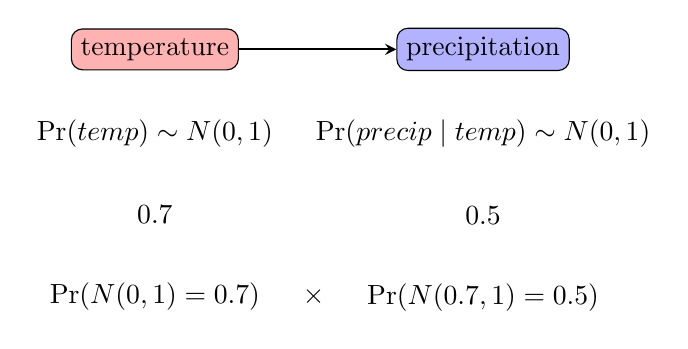
\begin{tikzpicture}
            \node [rectangle, rounded corners, draw, fill=red!30!white] 
            (t) {temperature};
            \node [rectangle, rounded corners, draw, fill=blue!30!white,
            right=2 of t] (p) {precipitation};
            \draw [->, >=stealth, thick] (t) -- (p);

            \uncover<2-> {
            \node [below=0.5 of t] (t1) {$\Pr(\text{temp}) \sim N(0, 1)$};
            \node [below=0.5 of p] (p1) {$\Pr(\text{precip} \mid \text{temp}) \sim N(0, 1)$};
            }

            \uncover<3-> {
            \node [below=0.5 of t1] (t2) {$0.7$};
            \node [below=0.5 of p1] (p2) {$0.5$};
            }

            \uncover<4-> {
            \node [below=0.5 of t2] (t3) {$\Pr(N(0, 1) = 0.7)$};
            \node [below=0.5 of p2] (p3) {$\Pr(N(0.7, 1) = 0.5)$};
            \path (t3) -- node {$\times$} (p3);
            }
        \end{tikzpicture}
    \end{center}
\end{frame}

\begin{frame}{Networks for QTLs}
    \begin{itemize}
        \item \textit{deal} and \textit{CGBayesNets} packages to construct one
            Bayesian network for each multi-QTL by exhaustive search
        \uncover<2->{
        \item With \textit{deal}, edges into genotype were blacklisted
        }\uncover<3->{
        \item Most common network structure was independence
        }\uncover<4->{
        \item Accounted for 42\% of \textit{deal} networks, 29\% of
            \textit{CGBayesNets} networks
        }
    \end{itemize}
    \begin{center}
        %       [g][e|g][ace|g][me|g] 101
%    [g][e|g][ace|e:me][me|g]  14
%      [g][e|g][ace|me][me|g]  13
%       [g][e|g][ace|e][me|g]  12
%      [g][e|me][ace|g][me|g]  12
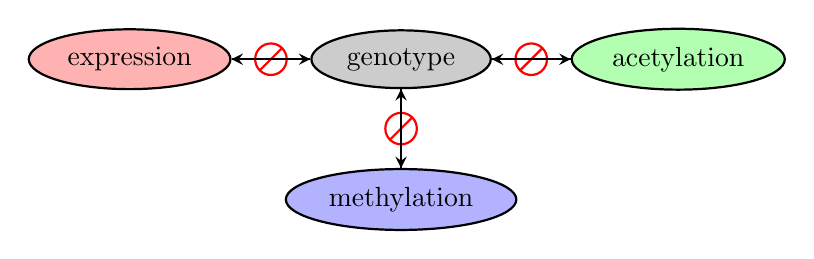
\begin{tikzpicture}
    [every node/.style={ellipse, draw, minimum width=8mm},
     every path/.style={->, >=stealth, thick, draw}]
    \node [fill=black!20!white] (g) {genotype};
    \node [fill=red!30!white, left=of g] (e) {expression};
    \node [fill=green!30!white, right=of g] (a) {acetylation};
    \node [fill=blue!30!white, below =of g] (m) {methylation};

    \uncover<2>{
        \draw (e) -- node [-, draw=red, minimum width=4mm, forbidden sign] { } (g);
        \draw (a) -- node [-, draw=red, minimum width=4mm, forbidden sign] { } (g);
        \draw (m) -- node [-, draw=red, minimum width=4mm, forbidden sign] { } (g);
    }

    \uncover<3->{
        \draw (g) -- (e);
        \draw (g) -- (a);
        \draw (g) -- (m);
    }
\end{tikzpicture}

    \end{center}
\end{frame}
\tikzexternalenable

\begin{frame}{Future Work}
    \begin{itemize}
        \item Expand the number of multi-QTLs
            \begin{itemize}
                \item More that just the best SNP per feature
                \item Identify overlapping QTLs intelligently
            \end{itemize}
        \item More rigourous criterion for number of PCs to remove
        \item Try other packages for network learning (HyPhy)
        \item Are QTLs enriched in SNPs identified in GWAS studies?
        \item Correlations with phenotype (cognitive decline etc.)
    \end{itemize}
\end{frame}

\begin{frame}{Thank you!}
    \begin{columns}
        \begin{column}{0.5\textwidth}
            \small
            \textbf{Harvard / Broad}
            \begin{itemize}
                \setlength\itemsep{-2pt}
                \item Philip L. D. Jager
                \item Lori Chibnik
                \item Jishu Xu
                \item Charles White
                \item Cristin McCabe
                \item Towfique Raj
            \end{itemize}
            \textbf{Rush}
            \begin{itemize}
                \setlength\itemsep{-2pt}
                \item David A Bennett
                \item Chris Gaiteri
                \item Lei Yu
            \end{itemize}
            \textbf{Bioinformatics Training Program}
            \begin{itemize}
                \setlength\itemsep{-2pt}
                \item All the students
                \item Sharon Ruschkowski
            \end{itemize}
        \end{column}
        \normalsize
        \begin{column}{0.5\textwidth}
            \begin{center}
                
\includegraphics[scale=0.3]{doc/logos/cmmt} \\
                \hfill\\
                
\includegraphics[scale=0.2]{doc/logos/bioinfo} \\
                \hfill\\
                
\includegraphics[scale=0.2]{doc/logos/ubc} \\
                \hfill\\
                
\includegraphics[scale=0.1]{doc/logos/nserc} \\
                \hfill\\
                
\includegraphics[scale=0.1]{doc/logos/broad} \\
                \hfill\\
                
\includegraphics[scale=0.1]{doc/logos/rush}
            \end{center}
        \end{column}
    \end{columns}
\end{frame}

\begin{frame}{Software}
    \begin{columns}
    \begin{column}{0.4\textwidth}
    \textbf{QTL analysis}
    \begin{itemize}
        \item
            \href{http://www.bios.unc.edu/research/genomic_software/Matrix_eQTL}
            {Matrix eQTL}
        \item
            \href{http://www.bioconductor.org/packages/release/bioc/html/qvalue.html}
            {qvalue}
    \end{itemize}
    \textbf{Bayesian networks}
    \begin{itemize}
        \item \href{http://cran.r-project.org/web/packages/deal/index.html}
                   {deal}
        \item \href{http://www.cgbayesnets.com}{CGBayesNets}
    \end{itemize}
    \end{column}
    \begin{column}{0.4\textwidth}
    \textbf{Slides}
    \begin{itemize}
        \item \href{http://www.ctan.org/pkg/beamer}{beamer}
        \item \href{https://www.ctan.org/pkg/pgf}{TikZ}
        \item
            \href{http://cran.r-project.org/web/packages/tikzDevice/index.html}
            {tikzDevice}
    \end{itemize}
    \textbf{Plots}
    \begin{itemize}
        \item \href{http://cran.r-project.org/web/packages/pheatmap/index.html}
                   {pheatmap}
        \item \href{http://ggplot2.org/}{ggplot2}
        \item
            \href{http://cran.r-project.org/web/packages/VennDiagram/index.html}
            {VennDiagram}
    \end{itemize}
    \textbf{Colour Scheme}
    \begin{itemize}
        \item \href{http://ethanschoonover.com/solarized}{solarized}
    \end{itemize}
    \end{column}
    \end{columns}
\end{frame}

\end{document}
